\documentclass{ltjsbook}
\usepackage{docmute} 
\usepackage{../../myStyle} 

\begin{document}
\chapter{二群の平均値差}
\label{Ch16_ttest}

心理学の実践で最もよく用いられるのが，平均値差の検定です。

本講ではまず，二群の平均値差の検定を考えます。「実験群(操作した群)」と「統制群(操作しなかった群)」に分けることで，平均値に差が見られたということは操作の効果があったと判断する，という考え方です。

この平均値差の検定は，\textbf{対応がある}場合と\textbf{対応がない}場合で分けて考える必要があります。対応がある，というのは2つの群のデータを得る時，背後に相関が考えられるケースを指します。対応がないというのは相関が考えられない場合です。無作為に実験群と統制群に振り分けた場合，この2群のデータに相関を考えることはできません(どの点とどの点をペアにしていいかわからないし，ペアにする意味もないので)。逆に2群の各点をペアにする意味がある場合，例えば事前・事後というように同じ人から2回データを取った場合とか，双子や``親密な関係''\footnote{恋人同士や夫婦関係のことを，社会心理学では一般的に「親密な関係」と表現します。持って回った言い方ですが，性別に限定されない良い表現だと思います。}のように元々相関があると考えられる場合は，対応があると考えます。

対応がある二群の場合は実はひとつの「差の分布」についての判断になるため，これまでと同様の議論ができます。対応がない二群の場合は，線形モデルの最も単純な場合でもあります。順に見ていきましょう。

\section{対応のある二群の平均値差の検定}

まずはプレ・ポスト(事前・事後)のデータを取った研究を例に考えましょう。たとえば心理的な健康状態について，事前にアンケート調査をしておき，その後なんらかの臨床的介入(リラックス法のトレーニングをする，など)を行って，一定期間後に同じ人に事後のアンケートを取る，というような研究デザインです(図\ref{fig:16_01})。

\begin{figure}[ht]
	\centering
	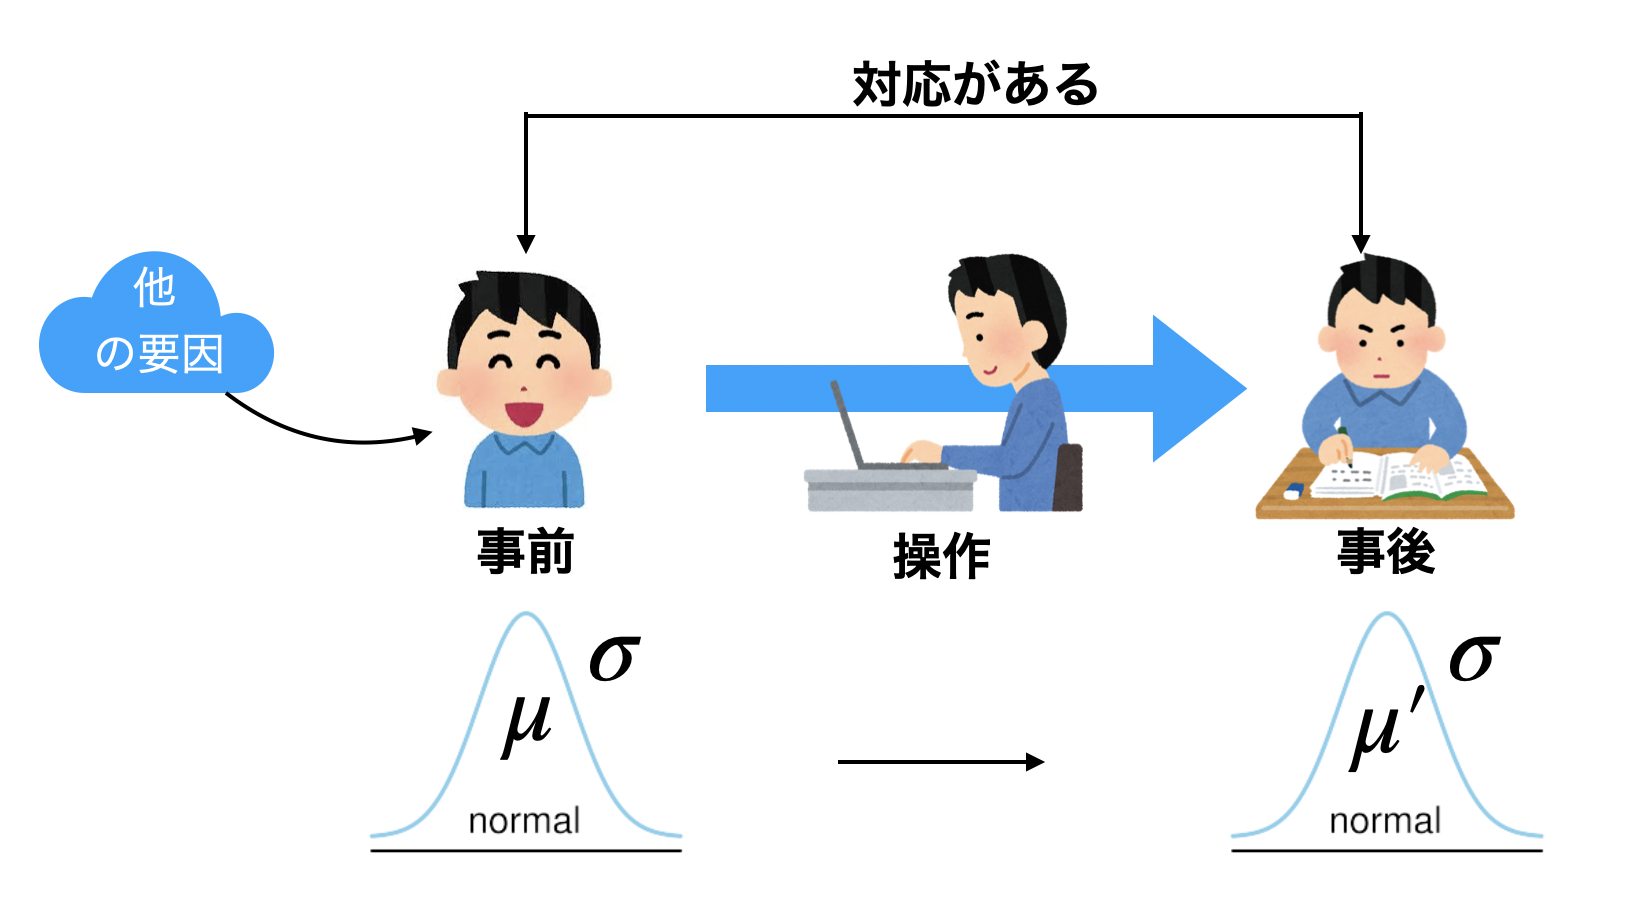
\includegraphics[keepaspectratio,width=0.8\linewidth]{figures/16_ttest/paired_design.png}
	\caption{対応のある二群の平均値差の検定のシーン}
	\label{fig:16_01}
\end{figure}

事前に集められた被験者は母集団から無作為に集められているとし，事前調査による健康状態のスコアが正規分布にしたがっていたとします。これと同じテストを事後に行ったとすると，個人差はあるにせよ全体的に効果があれば，この臨床的介入法は優れている，と言えそうです。個々のクライアントの変化も重要ですが，より効果を一般的に解釈するためには，推測統計学の力を借りて，母集団での変化，母平均の差を検証したいと考えるのは当然でしょう。そこで，標本平均から母平均を推定し，また母集団分布が正規分布であるという仮定をおくことで標本平均のブレ幅も想定できますから，これを使って母平均のありそうな場所を推定，それが事前・事後でどう違うかということを考えていきたいと思います。またここで，母平均はもちろん母SDもわからないので，標本から計算した不偏分散を推定値として考えます。標本統計量から推定する場合は，正規分布ではなく$t$分布に従いますので，ここでも$t$分布を使った推定をすることになります。この推定値を使った検定を考えるのですが，とくにこの検定のことを\keyterm{t検定}{tけんてい}{t-test}といいます\footnote{$t$分布を使った検定なので，$t$検定です。実は平均の差の検定意外にも$t$分布を使った推定・検定は多くあるのですが，非常に応用例の多いパターンですので，2群の平均値差の検定のことをt検定ということがあるのです。ちなみにこの時のtは小文字であることにご注意を。大文字のTは別の検定の時に使ったりします。ややこしい。}。


さて，事前・事後で変化があったかどうかを知りたいのですが，ありがたいことに正規分布に従う確率変数$X$と，正規分布に従う確率変数$Y$の差，$X-Y$も，正規分布に従うことがわかっています。今回はデータに対応があり，事前と事後で変化があったかどうかが知りたいわけですから，この特徴を使うことができます。

数値例として，次のような2群を考えてみましょう(表\ref{tbl:16_01})。
% latex table generated in R 4.0.2 by xtable 1.8-4 package
% Wed Sep  2 09:32:58 2020
\begin{table}[ht]
	\centering
	\caption{Pre-Post Design Data}
	\begin{tabular}{rrrrrrrrrrr}
		\hline
		Participants & 1  & 2  & 3  & 4  & 5  & 6  & 7  & 8  & 9  & 10 \\
		\hline
		pre          & 34 & 25 & 13 & 21 & 13 & 26 & 19 & 12 & 19 & 19 \\
		post         & 35 & 30 & 16 & 27 & 20 & 28 & 16 & 14 & 18 & 21 \\ \hline
		diff         & 1  & 5  & 3  & 6  & 7  & 2  & -3 & 2  & -1 & 2  \\
		\hline
	\end{tabular}
	\label{tbl:16_01}
\end{table}
ここには10人の実験参加者(participants)がいます。表\ref{tbl:16_01}には，それぞれの人の事前・事後のスコアと，その差分について示されています。数式で表しておきますと，まず事前のスコアを$X_1$,事後のスコアを$X_2$とします。すると差分$D$は
\[ D = X_2 - X_1 \]
ですが，その平均についても
\[ \bar{D} = \bar{X_2} - \bar{X_1} \]
という関係が成り立ちます。そしてこの$D$が，平均$\mu_D$，標準偏差$\sigma_D$の正規分布に従いますから，
\[ D \sim N(\mu_D,\sigma_D)\]
より
\[ \bar{D} \sim N(\mu_D,\frac{\sigma_D}{\sqrt{n}}) \]
ということになります。ここで$\sigma_D$がわかればいいのですが，わからないので$D$の不偏分散をその推定値としますと，
\[ t = \frac{\bar{D}-\mu_D}{\hat{\sigma_D}/\sqrt{n}} \]
と自由度$n-1$の$t$分布に従うことになるわけです。この一連の流れ，数式で表されるとピンとこないという人がいれば，第\ref{ch11_inference}講に立ち返って，確認してください。

さて，検定の前に区間推定してみましょう。自由度$n-1=10-1=9$の$t$分布の95\%区間は$\pm 2.262157$ですから\footnote{念のために書いておくと，Rで\texttt{qt(0.975,df=9)}とします。}，今回の数字を使って考えると，
\[ -2.262 < \frac{\bar{D}-\mu_D}{\hat{\sigma_D}/\sqrt{n}} < 2.262 \]
から，両辺に分母をかけて
\[ -2.262 \times \hat{\sigma_D}/\sqrt{n} < \bar{D}-\mu_D < 2.262 \times \hat{\sigma_D}/\sqrt{n} \]
$\bar{D}$を移項して
\[ \bar{D}-2.262 \times \hat{\sigma_D}/\sqrt{n} < \mu_D < \bar{D}+2.262\times \hat{\sigma_D}/\sqrt{n} \]
ここで$\bar{D} = 2.400,\hat{\sigma_D} = 3.062$ですから，
\[ 0.2097 < \mu_D < 4.590 \]
ということがわかります。標本の差分は2.4点だったのですが，母平均の差は点推定で2.4，95\%の区間推定で[0.21,4.59]ぐらいだということでした。つまり，95\%の幅で低く見積もっても，0.21以上ではあるわけですから，差がないわけではない，ということがわかります。

これを検定のロジックに乗せて考えてみましょう。
\paragraph{仮説の設定}帰無仮説と対立仮説が必要ですが，帰無仮説はないないづくし，前後の差がない，効果がないという仮説になります。記号を使っていうなら，$\mu_D=0$です。対立仮説は臨床的な効果があった，ということになりますから，従属変数の差は0プラスであるはず。つまり$\mu_D > 0$です。
\paragraph{検定統計量を選択}平均値の推定ですので，検定統計量は$t$ですね。
\paragraph{判断の基準になる確率を設定}有意水準$\alpha$，今回も5\%で勝負を決めるとしましょう。
\paragraph{検定統計量の実現値を計算}先ほどは区間推定をしたので$\frac{\bar{D}-\mu_D}{\hat{\sigma_D}/\sqrt{n}} $の計算はしていませんでした。しておきましょう。\underline{帰無仮説に従うなら，$\mu_D=0$なのですから}，
\[t= \frac{\bar{D}-\mu_D}{\hat{\sigma_D}/\sqrt{n}}  = \frac{2.4-0}{3.062/\sqrt{10}}  = 2.479\]
この$t = 2.479$は自由度$9$の$t$分布に従います。この実現値以上の$t$値が出てくる確率は，$p=0.0175$です。
\paragraph{最初に定めた仮説を支持するかどうかを判断}
判定基準5\%より小さい数字ですので，帰無仮説の下で計算したこの$t$の値は，珍しいと言えます。こんな珍しいことが生じたのだから，仮定が何か間違っている。つまり，差がないというのがおかしい。帰無仮説を棄却して，対立仮説を採択する，と判断します。

結果の報告の仕方は，
\begin{quote}
	対応のある$t$検定を行ったところ，$t(9)=2.479,p=0.0175$で統計的に有意である。
\end{quote}
ということになります。

ところで，先ほどの区間推定の結果を覚えているでしょうか？ 95\%の幅で考えると，少なく見積もっても0.21，大きく見積もると4.59も差があったかもしれません。この「少なく見積もっても」の方がゼロ(=帰無仮説)ではありませんので，この区間をみるだけでも帰無仮説を棄却することがわかります。この区間推定がゼロを挟む，つまり少なく見積もるとマイナス(逆効果！)，大きく見積もるとプラスだ，というときは検定をしても有意にはなりません。この区間推定の情報は，推定された平均値がどれほど変化しうるのか，の情報でもありますから，この大きさを一緒に報告しておくと「この実験がどれほど信用できるか」という目安にもなって良いですね。そこで先ほどの報告例を少し修正して，

\begin{quote}
	対応のある$t$検定を行ったところ，$t(9)=2.479,p=0.0175，95\%C.I.[0.21,4.59]$で統計的に有意である。
\end{quote}

とすると尚良いでしょう\footnote{5\%水準でカットするのも，95\%水準の幅を報告するのも，同じ情報で冗長だ，と思われるかもしれません。実にその通りで，かつ，帰無仮説検定の「有意差あり」という報告は信頼区間をみればわかる一方，その逆は成立しない($p$値は分布に関する情報ではない)のですから，有意差あり/なしという言い方は必要ないのです。今でもこの表現が使われるのは，旧世紀の名残でしかありません。}。

\subsection{検定と方向性}

ここで一つ注意をしておきます。今回の対立仮説は，$\mu_D > 0$でした。これはスコアが「健康状態」を表しており，大きな値の方がより健康であるということを意味していること，また臨床的介入によって「改善」されるのであるから，スコアが上がるはずであるということから必然的に出てくる仮説といえます。もしスコアが「不健康状態」「抑うつ度」などを表すものであれば，臨床的介入によってスコアは下がるはずですから，対立仮説は$\mu_D < 0$となるでしょう。

あるいは値の大小に意味がなく，とにかく「変化があるかどうか」だけに興味がある場合もあります。この場合は，$\mu_D \neq 0$という対立仮説を立てることになります。

このように，仮説の立て方には「方向性」がある場合とない場合があります。この方向性によって，検定統計量の判断が変わってきます。

今回は検定統計量の実現値を計算では，分子が$D = 2.4$であり，$t=2.479$でした。この$t$値が自由度9の$t$分布に従うことはわかっています。そこでこの値以上の$t$値が出る確率を計算したのですが，Rで\texttt{1-pt(2.479,df=9)}とすると，$p=0.0175$と出てきます。これは図\ref{fig:16_03}の上のように，2.479より右側の面積を求めたことになります。これが$\mu_D > 0$という対立仮説を立てた場合です。

前者を\keyterm{片側検定}{かたがわけんてい}{one sided test}，後者を\keyterm{両側検定}{りょうがわけんてい}{two sided test}と言います。これは図\ref{fig:16_03}を見るとわかりやすいです。ここには自由度9の$t$分布が描かれています。
\begin{figure}[ht]
	\centering
	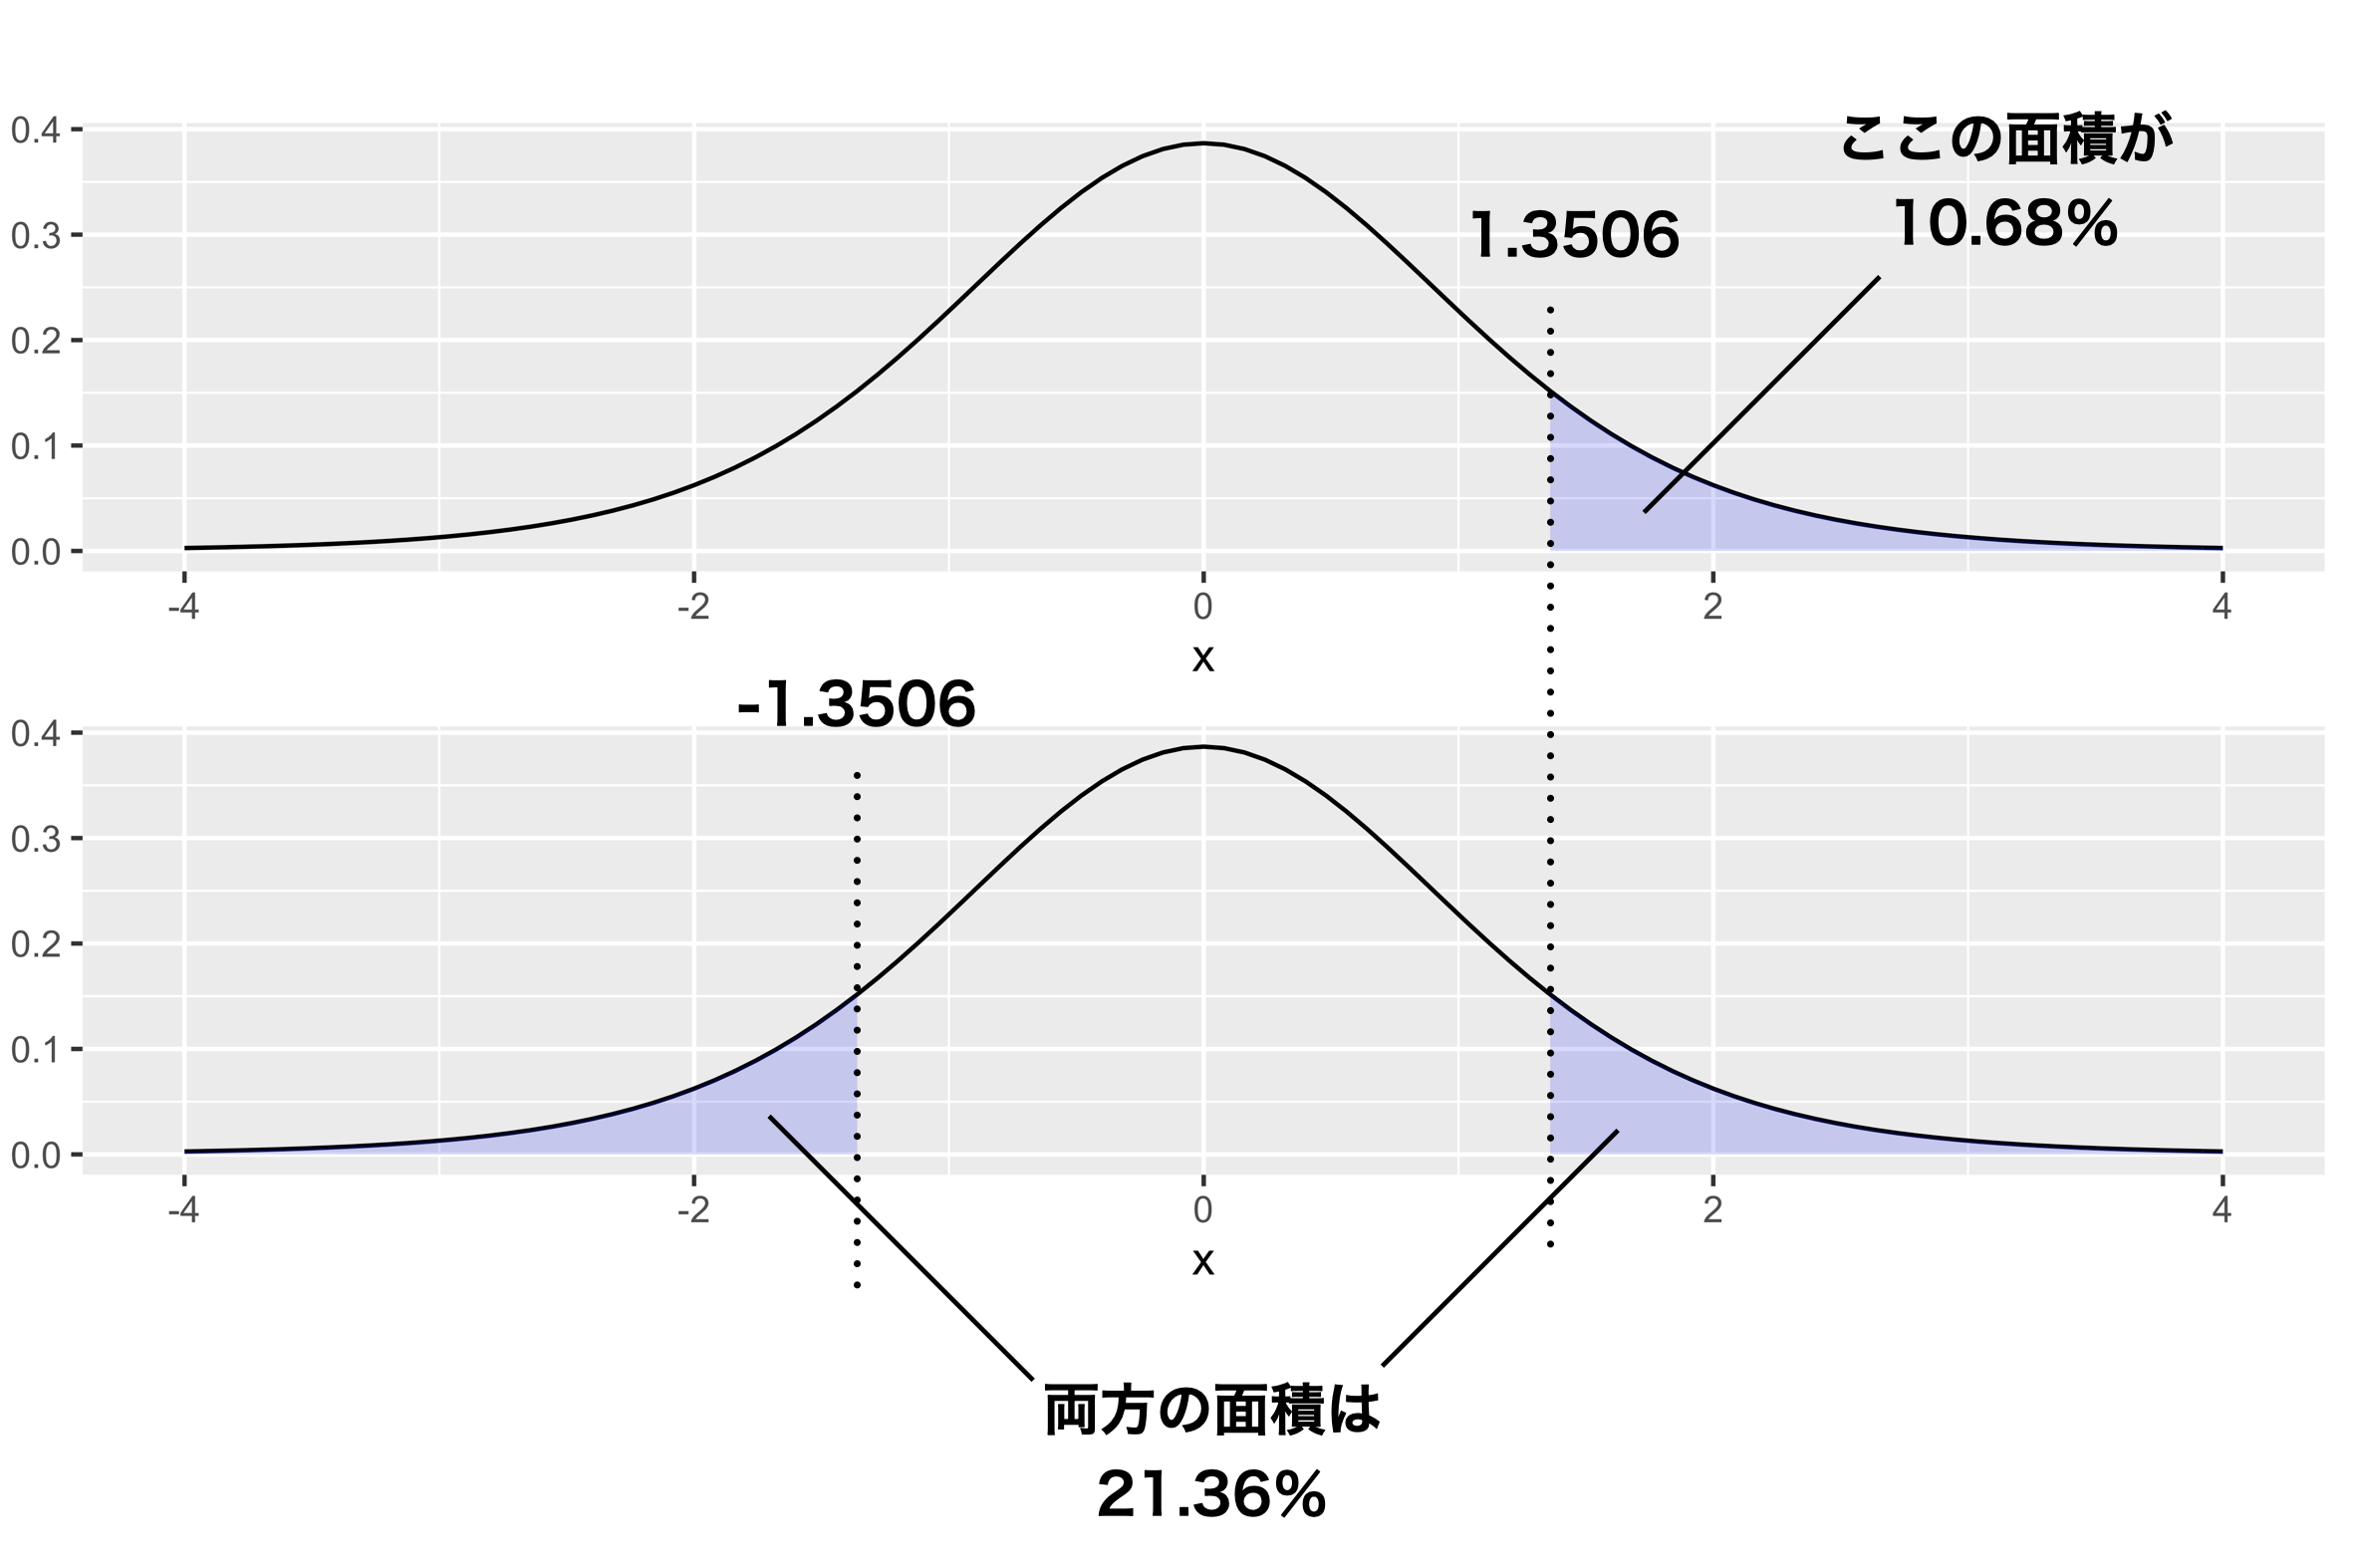
\includegraphics[keepaspectratio,width=0.8\linewidth]{figures/16_ttest/direction_of_test.png}
	\caption{片側検定(上)と両側検定(下)}
	\label{fig:16_03}
\end{figure}

今回は上のケース，すなわち変化の方向性に意味がある，片側検定の場合です。この図の色付けられたエリアは\keyterm{棄却域}{ききゃくいき}{rejection region}といい，この面積が全体の5\%になっています。今回の$t=2.479$はこのエリアに入っていますから，帰無仮説が棄却され，対立仮説が採択されます。臨床的介入の効果は，5\%水準で統計的に有意である，と判断できるのです。ちなみに，判断基準になる$t$値は，Rで\texttt{qt(0.95,df=9)}として，$1.833113$であることがわかります。この値を越えれば5\%水準で有意，ということになる判定ラインですね。この判定ラインのことを特に\keyterm{臨界値}{りんかいち}{critical value}と言います。

さて，では検定の方向性に意味がない場合はどうでしょうか。例えば錯視のように，大きく見えることもあれば小さく見えることもある，つまりどっちにしろ違いが出れば良い，というような場合です。対立仮説が$\mu_D \neq 0$であるこの時，同じ5\%でも棄却域はt分布の両側(図の下)で考えることになります。そうすると，上下に2.5\%ずつ，合計5\%のエリアが棄却域になります。臨界値は97.5\%点と2.5\%点の2つが必要になります。Rで\texttt{qt(0.975,df=9)}を計算すると，$2.262157$であり，このt分布は左右対称ですから，2.5\%点は$-2.262157$です。今回の$t$値は2.479ですから，両側で計算しても臨界値をこえ，棄却域に入っていますから，判断は変わりませんが，両側検定の方がより厳しい基準であることはわかると思います。

心理学研究の実践では，両側検定が行われることが多いです。実際，統計パッケージもデフォルトでは両側検定をするようになっています。厳しい方がデフォルトだからいいだろ，という考えもあるかもしれませんが，不用意に厳しくすることは研究実践としてやはりおかしなことで，
今回のように仮説に意味がある場合は片側検定で構いません。




\section{対応のない二群の平均値差の検定}
\subsection{区間推定でまず考えてみよう}
それでは次に，対応のないバージョン，つまり群間(Between)計画の例を考えてみましょう。これは両群に対応がない，それぞれの平均値の推定をして，その上でその推定値の間に差があるかどうか，という話になります。

\begin{figure}[ht]
	\centering
	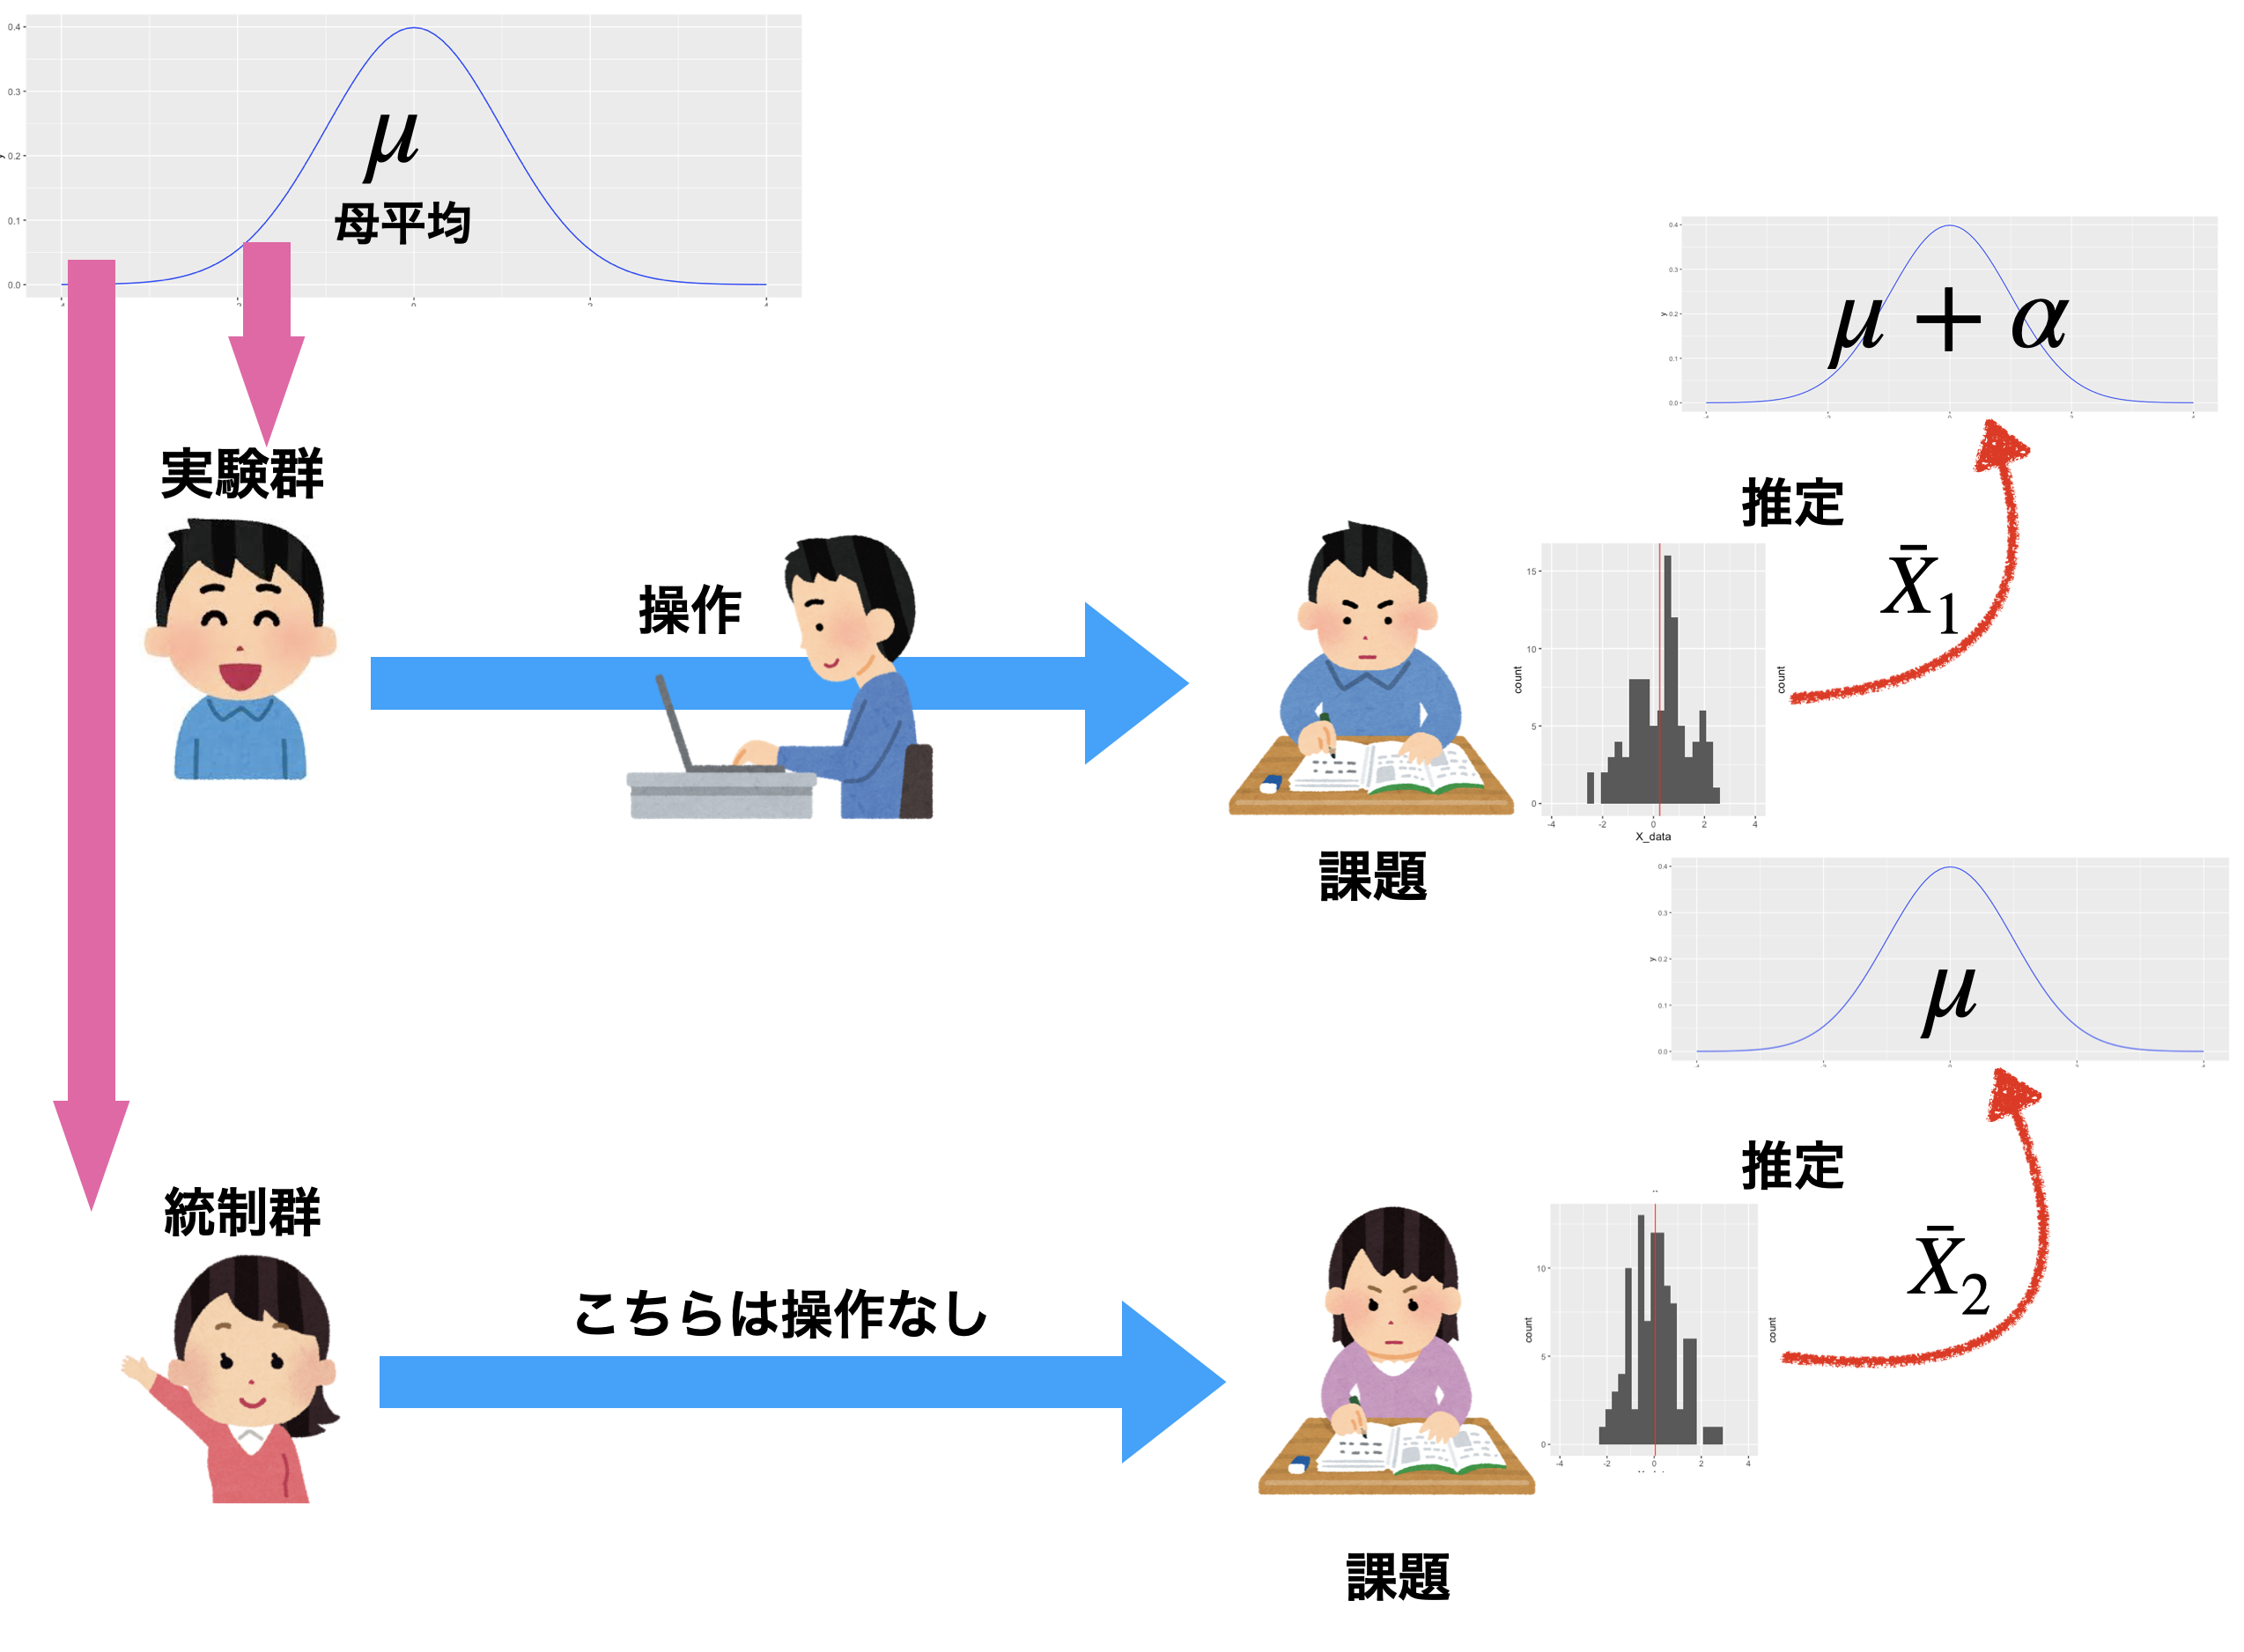
\includegraphics[keepaspectratio,width=0.8\linewidth]{figures/16_ttest/independent_t.png}
	\caption{対応のない二群の平均値差の検定のシーン}
	\label{fig:16_02}
\end{figure}

具体的な数値例でみてみましょう。
% latex table generated in R 4.0.2 by xtable 1.8-4 package
% Wed Sep  2 10:43:49 2020
\begin{table}[ht]
	\centering
	\caption{Between Designのデータ例}
	\begin{tabular}{rlr}
		\hline
		ID & condition    & value \\
		\hline
		1  & control      & 25    \\
		2  & control      & 15    \\
		3  & control      & 24    \\
		4  & control      & 17    \\
		5  & control      & 22    \\
		6  & experimental & 31    \\
		7  & experimental & 28    \\
		8  & experimental & 30    \\
		9  & experimental & 19    \\
		10 & experimental & 18    \\
		\hline
	\end{tabular}
	\label{tbl:16_02}
\end{table}
今回は$n=5$としました。5人の実験参加者を実験群(experimental)と統制群(control)に無作為に割り付け，実験群にはある認知課題を課した後で，記憶力を測定するテストをした，と思ってください。テストのスコアがvalue列に入っている数字です。さて，認知課題をした群とそうでない群の平均値に違いはあるでしょうか？

これまた母SDがわからない中で，標本平均から母平均を推定するので$t$分布を使うことになります。実験群，統制群ともに$n=5$ですから，自由度$n-1=5-1=4$の$t$分布を使って推定すると，統制群の母平均は
$\bar{X}_{ctl} =20.60$,$\hat{\sigma_{ctl}}=4.393$より，
\[15.145 < \mu_{ctl}<26.055 \]
となります。実験群は$\bar{X}_{exp} = 25.20$,
$\hat{\sigma_{exp}}=6.221$より
\[17.476<\mu_{exp}< 32.924 \]
となります。

差がありますか？ 微妙ですね！統制群は大きく見積もるなら26.05ぐらいの標本平均が出てきたかもしれなかったし，実験群は小さく見積もるなら17.48ぐらいの標本平均だったかもしれないわけです。区間推定だけだと判断に迷うところです。

\subsection{検定で勝負を決める}
そこで検定の出番。先ほどの例と同じく，「正規分布と正規分布の引き算はまた，正規分布」という特徴を利用して検定を行います。正規分布である母集団$N(\mu,\sigma)$から無作為標本を取ってきたとすると，標本平均$\bar{X}$は$N(\mu,\frac{\sigma}{\sqrt{n}})$に従うのでした。ここで，2つの群の標本平均の差，$\bar{X}_1 - \bar{X}_2$を考えると，その分布は平均$\mu_1-\mu_2$，標準偏差$\sigma/\sqrt{\frac{1}{n_1}+\frac{1}{n_2}}$に従うことがわかっています。ただ，この$\sigma$がわかりませんので，不偏推定量で置き換える必要があります。今回は2つの群があって，実験群の不偏分散を使っても，統制群の不偏分散を使ってもおかしいので，両群をまとめて
\[ \hat{\sigma^2}_{pooled} = \frac{(n_1-1)\hat{\sigma_1^2}+(n_2-1)\hat{\sigma_2^2}}{n_1+n_2 - 2}\]
を使います。pooledとはプールした，まとめた，という意味です。これは分散の推定量ですから，差の分布の標準偏差の推定値としてはこれの正の平方根，
\[ \hat{\sigma}_{pooled} = \sqrt{\frac{(n_1-1)\hat{\sigma_1^2}+(n_2-1)\hat{\sigma_2^2}}{n_1+n_2 - 2}}\]を使えば良いことになります。

ややこしくなってきましたが，これを使って考えると統計量は次のように計算できます。

\[ t = \frac{\bar{X_1}-\bar{X_2}-(\mu_1-\mu_2)}{\sqrt{\frac{(n_1-1)\hat{\sigma_1^2}+(n_2-1)\hat{\sigma_2^2}}{n_1+n_2 - 2}}\sqrt{\frac{1}{n_1}+\frac{1}{n_2}}}\]

あっ，心を閉ざさないで！数式は話の筋を通すために書いているだけです。文字がいっぱい出てきて混乱したかもしれませんが，この数式，覚えておく必要はありません。ここでは，教材なので一応説明していきますが，実際には統計ソフトウェアが組み込まれた関数で一気に答えを出してくれます。大事なのは，筋道を理解することですので，初めのうちは数式のところは「なんか書いてるわ」ぐらいの理解でも構いません。それよりも，この$t$の式には標本統計量しか入っていないことに感動しましょう。

「うそつけ，$\mu_1,\mu_2$があるじゃないか」と思った人は，目の付け所がいいですね。確かにこれはわからないところ(だからギリシア文字で書いてあります)なのですが，これを使って今から検定を行うのです。検定では帰無仮説をおきます。帰無仮説はないないづくし，ですから，「2群の母平均の間に差はない」と仮定するのです。これを言葉でいうと，$\mu_1=\mu_2$，あるいは$\mu_1-\mu_2=0$です。上手くできてますよね！帰無仮説の下では，分母の$\mu_1-\mu_2$を$=0$とおくことができますので，
\[ t = \frac{\bar{X_1}-\bar{X_2}}{\sqrt{\frac{(n_1-1)\hat{\sigma_1^2}+(n_2-1)\hat{\sigma_2^2}}{n_1+n_2 - 2}}\sqrt{\frac{1}{n_1}+\frac{1}{n_2}}}\]
となり，完全に標本統計量から計算できることになりました。それでは検定を進めて参りましょう。
\paragraph{仮説の設定}帰無仮説と対立仮説が必要です。先ほども述べたように，帰無仮説は$\mu_1=\mu_2$，対立仮説はこれの否定ですので$\mu_1 \neq \mu_2$になります。両側検定になっていることに注意してください。
\paragraph{検定統計量を選択}平均値の推定ですので，検定統計量は$t$ですね。
\paragraph{判断の基準になる確率を設定}有意水準$\alpha$，今回も5\%で勝負を決めるとしましょう。
\paragraph{検定統計量の実現値を計算}これはちょっと厄介ですが，数式にしたがって，統制群を$X_1$，実験群を$X_2$とおくと，$\bar{X_1}=20.60,\hat{\sigma}_1=4.393,\bar{X_2}=25.20,\hat{\sigma}_2=6.221$です。

\[ t = \frac{20.60-25.20}{\sqrt{(4.393^2+6.221^2)/5}} = -1.3506\]

となりましたので，これが自由度$(n_1-1)+(n_2-1)=n_1+n_2-2=10-2=8$の$t$分布に従うことになります。これより極端な$t$値が得られる確率は，$p=0.1068$になりました。

\paragraph{最初に定めた仮説を支持するかどうかを判断}
判定基準5\%より大きい数字ですので，帰無仮説の下で計算したこの$t$の値は，珍しいとは言えません。

報告する時は次のようになります。今回は両側検定ですので$t$値の絶対値を使います。
\begin{quote}
	実験群と統制群の平均値の差を検定したところ，$t(8)=1.356,p=0.214$で統計的に有意であるとは言えなかった。
\end{quote}

2群の平均値の差の検定については，このような手続きで行います。繰り返しになりますが，実際の計算は機械がやってくれるので，どのような数字がどのような意味を持っているのか，得られた結果からどのように判定するのか，という手続き的な知識をしっかりと踏まえてください。

また，ここでこのように検定の具体例をみてきたわけですから，是非この技術を身の回りでも活用してみてください。

何か2つのグループがあって，その平均値が違うのであれば，これは偶然によるものなのかそうでないのか。一般化して良いのかどうか。この推測統計学的発想は，身の回りの至る所に応用できるものです。知識と技術を手に入れたら，是非具体例を自分で考えて，試してみてください\footnote{たとえば「お兄ちゃんのフライドポテトの方が，いつも長いのばっかり入っていてずるい！」というような兄弟喧嘩の種も，両者のフライドポテトの長さを測り，その平均値を出して$t$検定すれば「たまたま今回のポテトの問題だった」のか，いつもそうなる現象なのか検定で決着をつけることができます。実際に筆者が居酒屋のフライドポテトでこれの検証をした時，テーブルごとのポテトの長さに平均的な差はありませんでした。くわえて，フライドポテトの長さが非常に正規分布に近かったのを知って，感心したことがあります。}


\section{Rによる実践；対応のあるt検定}
では今度は手を動かして，Rでt検定を実際に行ってみましょう。
まずは対応のある\keyterm{t検定}{tけんてい}{t-test}です。面倒な計算式がありましたが，今回その辺の計算は機械がやってくれますので，例によって出力をしっかり確認するようにしましょう。

例として，表\ref{fig:16_01}の10人の参加者データを使います。元になるデータをオブジェクトに格納する\texttt{code:\ref{code:16_01}}を実行しましょう。
\begin{lstlisting}[language=c++,label={code:16_01},caption={t検定を行う}]
X <- c(34, 25, 13, 21, 13, 26, 19, 12, 19, 19)
Y <- c(35, 30, 16, 27, 20, 28, 16, 14, 18, 21)
t.test(Y, X, paired = T, alternative = "greater")
\end{lstlisting}

\paragraph{コード解説}
\begin{description}
	\item[1行目] 一方のデータをオブジェクト\texttt{X}に代入しています。\texttt{c}は結合combineという関数です。
	\item[2行目] 他方のデータをオブジェクト\texttt{Y}に代入しています。
	\item[3行目] t検定を行っています。引数として，データ\texttt{X,Y}を指定し，次に\texttt{paired}オプションを\texttt{T}に\footnote{大文字の\texttt{T}は$TRUE$，真であり，この逆は\texttt{F}とかいて$FALSE$,偽を意味する\textbf{特別な文字}です。真か偽か，本当か嘘かという2つの状態を表す論理値と呼ばれるもので，ここではスイッチオン/オフの意味です。対応スイッチ，オン！という意味ですね。大文字の$T,F$をオブジェクト名にして利用することも可能ですが，Rが専門的な意味で使う予約語なので，一般的にはそのような使用は避けた方が望ましいです。}，対立仮説alternativeを「YがXよりも大きい」という\underline{片側検定}にしてあります。
\end{description}

さて，こうして得られる結果は\texttt{Rの出力\ref{RS:out16_04}}の通りです。
\begin{Rscreen}{t.testの出力}{out16_04}
\begin{verbatim}
Paired t-test

data:  Y and X
t = 2.4783, df = 9, p-value = 0.01754
alternative hypothesis: true mean difference is greater than 0
95 percent confidence interval:
 0.6248331       Inf
sample estimates:
mean difference 
            2.4 
\end{verbatim}
\end{Rscreen}

上から三行目に$t$値が出ていますね。帰無仮説の下での$t$統計量の実現値は$t(9)=2.4783$であり，これが出現する確率は$p=0.01754$です。対立仮説は，平均値の差が0より小さい(true mean difference is greater than 0)という方向性のある対立仮説になっています\footnote{Rでは前の変数が後ろの変数に比べて大か，小かを表現しますので，Y,Xの順で書いています。}。これが片側検定になっているのは，\texttt{t.test}関数の引数に\texttt{alternative="greater"}と書いたからで，これを\texttt{alternative="less"}とすれば逆の片側検定(事後データのスコアの方が事前データのスコアより小さい)を検定することになり，とくに何も書かなないか，\texttt{alternative="two.sided"}とすれば両側検定になります。


\section{Rによる実践；対応のないt検定}
つづいて対応のない\keyterm{t検定}{tけんてい}{t-test}のほうも，Rでできるようになりましょう。

さきほどの表\ref{tbl:16_02}のデータを分析することを考えます。難しい計算は抜きにして，\texttt{code:\ref{code:16_03}}を入力し，分析を実行してください。
\begin{lstlisting}[language=c++,label={code:16_03},caption={formulaで指定}]
X <- c(25, 15, 24, 17, 22)
Y <- c(31, 28, 30, 19, 18)
dat <- data.frame(condition = c(rep(1, 5), rep(2, 5)), value = c(X, Y))
dat$condition <- factor(dat$condition, 
                        labels =  c("control","experimental"))
t.test(value ~ condition, data = dat)
\end{lstlisting}
スクリプトの内容については，先ほどとほぼ同じです。大きな違いは，\texttt{t.test}関数の引数がなくなったところで，\texttt{paired}オプションもなければ，\texttt{alternative}オプションもありません。ないのは，デフォルトの状態を使っているからで，Rの\texttt{t.test}関数はデフォルトで対応のない，両側検定の$t$検定をやってくれるのです。

結果は次のように表示されるはずです(\texttt{Rの出力\ref{RS:out16_05}})。
\begin{Rscreen}{Welchの補正}{out16_05}
	\begin{verbatim}
Welch Two Sample t-test

data:  value by condition
t = -1.3506, df = 7.195, p-value = 0.2178
alternative hypothesis: true difference in means is not equal to 0
95 percent confidence interval:
 -12.609577   3.409577
sample estimates:
     mean in group control mean in group experimental 
                      20.6                       25.2 
\end{verbatim}
\end{Rscreen}
前回，手計算した結果と同じになっているかどうか確認してください。

んん？ 自由度が7.195? 自由度って8になるんじゃなかったでしたっけ(実験群の自由度が$5-1=4$，統制群の自由度も$5-1=4$，足して2つで$4+4=8$)。

\subsection{Welchの補正}
そうです，t検定の自由度は$8$のはずなのですが，変な数字で出ていますね。これは，検定に関わるまだ説明していない別の手続きがあったからです。

検定にはどのような仮定があったか，思い出してください。母平均の差をゼロとする，という帰無仮説をおくのも仮定ではありますが，さらにその前にあった仮定です。それは，2つの群が正規分布から得られていること，とくに平均値に差はあるけれども，母標準偏差は同じところから取ってきていた，という仮定があったのです。

もしこの仮定が崩れていたら？ 母集団に正規分布が仮定できなければ，$t$検定はできません。たとえば年収の差とか，データが比率や角度についての数字であったりすると，正規分布を仮定できないので$t$検定はできないのです。正規分布は正規分布だったとしても，母標準偏差がちがっているなら，推定の仕方も考え直さないといけないかもしれません。

この問題は，$t$値の自由度を調整することで解決されています。前回までのいわゆる$t$検定は，等分散の仮定が満たされているケース(分散の均一性などということもあります)の計算方法であり，この仮定が満たされていない場合は\keyterm{Welchの補正}{Welchのほせい}{Welch's correction}(ウェルチの補正)とよばれる調整が必要です。

Rの\texttt{t.test}関数は，より仮定の緩やかな，Welchの補正をかけた結果をデフォルトで返してくれます。まず分散が等しいかどうかチェックして云々，という手続きが面倒なので，最初から補正しておこう，ということですね。結果の一行目にもWelch Two Sample t-testと書いてあります。これを使って，結果は
\begin{quote}
	$t(7.195)=1.351,p = 0.2178$で2群の間に統計的に有意な差は認められなかった。
\end{quote}
と報告します\footnote{$t$の値は，両側検定の場合符号に意味がないのでマイナスを取って記載します。}。差があるかどうかの判断だけでなく，差の95\%信頼区間にも目を向けておきましょう。結果から，差の95\%信頼区間はCI[-12.609577,3.409577]でした。差は-12から+3までの幅があり，帰無仮説である差$=0$を含んでいるので，有意になりません。


ところで，分散が同じだ，と仮定できる場合は\texttt{t.test}関数のオプションを使います(\texttt{code:\ref{code:16_04}})。

\begin{lstlisting}[language=c++,label={code:16_04},caption={分散のオプション指定}]
t.test(value ~ condition, data = dat,var.equal = T)
\end{lstlisting}

これで，\texttt{Rの出力\ref{RS:out16_06}}のような結果を得ることができます。

\begin{Rscreen}{分散が等しいという仮定を置く}{out16_06}
	\begin{verbatim}
	Two Sample t-test

data:  value by condition
t = -1.3506, df = 8, p-value = 0.2138
alternative hypothesis: true difference in means is not equal to 0
95 percent confidence interval:
 -12.453967   3.253967
sample estimates:
     mean in group control mean in group experimental 
                      20.6                       25.2 
\end{verbatim}
\end{Rscreen}
このやり方ですと，自由度も整数になっていますね(判定結果は変わりませんが)。

\subsection{事後的に効果量を検証する}
検定が終わった後ではありますが，このデータの実験は「勝ち目がある」ものだったのでしょうか。つまり，母集団における母平均の差が十分大きなものなのかどうかが気になります。母数は分かりませんが，これまでも分からないものは標本統計量で置き換えて推定してきたわけですから，データを取った後になって，これはどれぐらい効果量の大きなデータだったのか，を考えてみましょう。

効果量の計算についても，Rを使って簡単に行うことができます。Rではパッケージを追加することでさまざまな統計関数が増えますが，効果量についての\textsf{effsize}パッケージ\parencite{effsize}を導入すれば，この計算も簡単にできます。効果量については第\ref{ch14_NHST2}講で触れましたので確認しておいてください。ここではより推奨される，Hedgesのgの算出の仕方を紹介します(\texttt{code:\ref{code:16_05}})。

\begin{lstlisting}[language=c++,label={code:16_05},caption={効果量を求める}]
# パッケージの読み込み
library(effsize)
cohen.d(value ~ condition, data = dat, hedges.correction = T)
\end{lstlisting}
ここではまず2行目でパッケージを読み込み\footnote{このパッケージを持っていない場合は，当然インターネットからダウンロードしてローカル(手元のPC)に保存しておく必要があります。}，次の行でcohenのdをHedgesの補正をかけて算出せよ，としています。

結果は\texttt{Rの出力\ref{RS:out16_07}}のように示されます。
\begin{Rscreen}{効果量の出力}{out16_07}
	\begin{verbatim}
Hedges's g

g estimate: -0.7715342 (medium)
95 percent confidence interval:
       lower      upper 
-2.1369693  0.5939009 
\end{verbatim}
\end{Rscreen}

\texttt{g estimate: -0.7715342 (medium)}とあるように，推定値は0.77で，これは中ぐらい(medium)の大きさだよ，ということです。中程度の違いがありそうなのに，今回有意にならなかったのは，サンプルサイズが小さかったからかもしれません。事前にきちんと設計してやっておけば，実験手続きとしてより良くなったでしょう。

効果量の計算はこのように，事後的に行って今回の標本から標準化された平均値の差がどれぐらいありそうか，と考えることもできます。もちろん事前に平均値の差を想定して，そこから例数設計(どれぐらいのサンプルを取れば良いか考える)するのにも使います。今回ここで求めた標本効果量も，レポートに書くようにしましょう。

\begin{quote}
	$t(7.195)=1.351,p = 0.2178$で2群の間に統計的に有意な差は認められなかった。なお，Hedgesのgで効果量を求めたところ，0.77であった。
\end{quote}

\subsection{サンプルサイズの設計}
ところで今回，対応のない$t$検定で，効果量が0.7あるのに有意になりませんでした。これはサンプルサイズが小かったからかも，ということでしたが，では何人分のデータがあればよかったのでしょうか。\texttt{code:\ref{code:16_09}}ようにRに入力することで，そのヒントが得られます。
\begin{lstlisting}[language=c++,label={code:16_09},caption={power.t.test関数}]
power.t.test(power = 0.8, delta = 0.7, sig.level = 0.05)
\end{lstlisting}
ここで，\texttt{delta=0.7}としたのは，標準化された平均値差が0.7あるとして，という考え方です。これは先ほどの事後的検定力分析の結果，それぐらいあったんじゃないの？ と思われたのでその値を使いました。もっと小さく見積もったり，逆にもう少し大きく見積もったりしても構いません。また，\texttt{power=0.8}としましたが，これは\keyterm{検定力}{けんていりょく}{power}で，セクション\ref{TypeI_II_Error}(Pp.\pageref{TypeI_II_Error})で出てきたものです。Type II Error，つまり差があるのにあると言えない間違い($\beta$)を20\%ぐらいに抑え，80\%の確率で当てたいとしました($1-\beta=0.8$)。また，有意水準は5\%です($\alpha=0.05$,スクリプトの中では\texttt{sig.level=0.05}としています)。

さて，これの出力結果を見ると，次のように示されました(\texttt{Rの出力\ref{RS:out16_09}})。
\begin{Rscreen}{rnormの出力}{out16_09}
	\begin{verbatim}
Two-sample t test power calculation 

n = 33.02467
delta = 0.7
   sd = 1
sig.level = 0.05
power = 0.8
alternative = two.sided

NOTE: n is number in *each* group
\end{verbatim}
\end{Rscreen}
ここの$n$にあるように，効果量0.7，検定力0.8で研究するのであれば，33か34人は集めたいところ，だったわけです。逆に今回は5人しか集めていませんでしたが，これを使って，\texttt{code:\ref{code:16_10}}とすると，\texttt{Rの出力\ref{RS:out16_10}}のように示されます。

\begin{lstlisting}[language=c++,label={code:16_10},caption={power.t.testで$n$を固定}]
power.t.test(n = 5, delta = 0.7, sig.level = 0.05)
\end{lstlisting}

\begin{Rscreen}{検定力の出力}{out16_10}
	\begin{verbatim}
Two-sample t test power calculation 

n = 5
delta = 0.7
sd = 1
sig.level = 0.05
power = 0.16318
alternative = two.sided

NOTE: n is number in *each* group
\end{verbatim}
\end{Rscreen}
ここにあるように，検定力は0.16，つまりサンプルサイズ$n=5$であれば，この研究は100回やっても「有意差あり」と正しく判断できるのは16回ほどしかなかった，ということになります。分の悪い勝負に出たというところでしょうか。

第\ref{ch14_NHST2}講，\ref{sec:14_04}節(Pp.\pageref{sec:14_04})で，このような検定力分析についても触れましたが，帰無仮説検定で「有意になること」を目的にするのであればサンプルサイズを増やせば良いのです。しかしもちろん，自分に都合のいい結果になるように努力？するのは科学的な実践としては不適切ですし，サンプルをたくさん取るのは研究上の労力もかかります。多過ぎず，少なすぎず，正しく判断するためのサンプルサイズを事前に設計してから，研究を始めることが重要です。


\subsection{補遺}
\paragraph{対応のあるt検定の効果量を計算する}対応のある$t$検定をして，その効果量を求める場合は，次のようにpairedオプションをオンにしておきます(\texttt{code:\ref{code:16_06}})。

\begin{lstlisting}[language=c++,label={code:16_06},caption={cohenのd}]
cohen.d(X,Y,paired = TRUE)
\end{lstlisting}
ただし，チルダを使った書き方をしている場合，\texttt{code:\ref{code:16_07}}のようにすると，出力に次のような警告が付されます(\texttt{Rの出力\ref{RS:out16_08}})。
\begin{lstlisting}[language=c++,label={code:16_07},caption={cohenのdその2}]
cohen.d(value ~ condition, data = dat, paired = TRUE)
\end{lstlisting}

\begin{Rscreen}{rnormの出力}{out16_08}
	\begin{verbatim}
Cohen's d

d estimate: -0.344241 (small)
95 percent confidence interval:
      lower       upper 
-0.64457930 -0.04390272 

    警告メッセージ: 
cohen.d.formula(value ~ condition, data = dat, paired = TRUE) で: 
Trying to compute paired samples Cohen's d using formula input. Results may be incorrect
 if cases do not appear in the same order for both levels of the grouping factor. Use the
format 'value ~ treatment | Subject(id)' to specify a subject id variable.
\end{verbatim}
\end{Rscreen}
この警告は，「対応のある個々人を識別する変数がデータセットに入ってないので，間違った結果になっているかもしれませんよ。次の書式を使ってください」と言ってます。これに対応するためには，\texttt{code:\ref{code:16_08}}のようにします。
\begin{lstlisting}[language=c++,label={code:16_08},caption={対応のある場合のcohen.d}]
X <- c(34, 25, 13, 21, 13, 26, 19, 12, 19, 19)
Y <- c(35, 30, 16, 27, 20, 28, 16, 14, 18, 21)
dat <- data.frame(condition = c(rep(1, 10), rep(2, 10)), value = c(X, Y))
dat$condition <- factor(dat$condition, labels = c("pre", "post"))
dat$ID <- rep(1:10,2)
cohen.d(value ~ condition | Subject(ID), data = dat, paired = TRUE)
\end{lstlisting}
ここでのポイントは5行目にIDを識別する変数を作り\footnote{関数\texttt{rep}で\texttt{1:10}を2回繰り返しています。Rではコロンで繋げた数字は，連番を意味します。}，効果量を計算する式を警告の提案通りのフォーマットに書き換えています。

\section{課題}
次の計算をするRコードが含まれるRスクリプトファイルを提出してください。
% \paragraph{課題1 標本統計量と一標本検定}
% 表\ref{exe:20_1}のようなデータが得られたとして，次の各指示に従い，結果について回答してください。
% % latex table generated in R 4.0.2 by xtable 1.8-4 package
% % Fri Oct 16 12:52:58 2020
% \begin{table}[ht]
%     \centering
%     \caption{課題1}
%     \label{exe:20_1}
%     \begin{tabular}{rrrrrrrrrr}
%       \hline
%     56 & 57 & 49 & 45 & 56 & 32 & 56 & 47 & 47 & 41 \\ 
%        \hline
%     \end{tabular}
%     \end{table}
% \begin{enumerate}
%     \item このデータセットの標本分散を計算してください
%     \item このデータセットの不偏標準偏差を計算してください
%     \item このデータセットが正規分布に従う母集団から得られたと考えて，母平均について95\%の区間推定をしてください
%     \item このデータセットが母平均$\mu=50$の正規分布から得られたかどうか，5\%水準で検定してください
% \end{enumerate}

\paragraph{課題1 対応のあるt検定}
表\ref{exe:16_2}にあるように，ある介入の事前・事後の心理検査の成績が得られたとして，次の各指示に従い，結果について回答してください。
% latex table generated in R 4.0.2 by xtable 1.8-4 package
% Fri Oct 16 12:59:41 2020
\begin{table}[ht]
	\centering
	\caption{課題2}
	\label{exe:16_2}
	\begin{tabular}{rrrrrrrrr}
		\hline
		pre  & 19 & 38 & 24 & 25 & 12 & 28 & 11 & 17 \\
		post & 31 & 23 & 28 & 35 & 14 & 4  & 4  & 38 \\
		\hline
	\end{tabular}
\end{table}

\begin{enumerate}
	\item 事前スコアの方が事後スコアよりも低いかどうか，5\%水準で検定してください。
\end{enumerate}

\paragraph{課題2 対応のないt検定}
表\ref{exe:16_3}にあるように，統制群と実験群の心理検査の成績が得られたとして，次の各指示に従い，結果について回答してください。
% latex table generated in R 4.0.2 by xtable 1.8-4 package
% Fri Oct 16 13:05:51 2020
\begin{table}[ht]
	\centering
	\caption{課題3}
	\label{exe:16_3}
	\begin{tabular}{rrrrrrrrrrr}
		\hline
		Control      & 20 & 21 & 21 & 20 & 21 & 22 & 22 & 22 & 20 & 20 \\
		Experimental & 20 & 18 & 22 & 20 & 21 & 18 & 19 & 21 & 21 & 21 \\
		\hline
	\end{tabular}
\end{table}

\begin{enumerate}
	\item 母分散が等しいと仮定したt検定を実行してください。
	\item 母分散が等しいという仮定をおかないt検定を実行してください。
	\item この検定に関して，効果量としてHedgesのgを算出してください。
\end{enumerate}


\end{document}
